\chapter{Architecture}

% \instructions{
%     Describe the architecture of your software as covered in the SEP2 module. The main goal of this chapter is describing the \textbf{technical implementation} in a way that a new team member can start working on the product as fast as possible.
    
%     \begin{itemize}
%         \item Use an existing template as a starting point (\texttt{arc42}, \texttt{C4 model}, ...)
%         \item Focus on stable, high-level concepts rather than details
%         \item Cover different views (static, dynamic, deployment, ...)
%         \item Prefer diagrams over text (ideally UML)
%         \item Explain the reasons behind your actions: \textit{Why did we build it like this?}
%     \end{itemize}   
% }


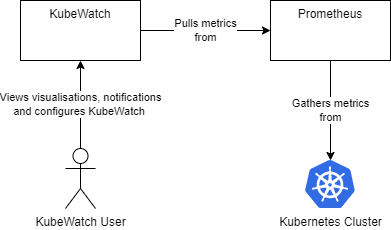
\includegraphics[height=6cm]{resources/System_context_diagram.png} \newline

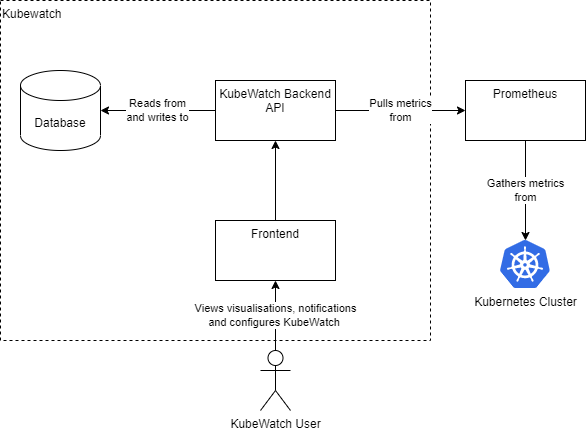
\includegraphics[height=8cm]{resources/Container_diagram.png}


\begin{tabular}{ll}
  \textbf{Master:}        & Each Kubernetes cluster contains at least one master node which runs the \\ 
                          & Kubernetes control plane. These control plane consists of an API server, \\
                          & scheduler, controller manager, etc. \\
  \textbf{Worker/Node:}   & Each cluster includes at least one worker node, this node runs containerized \\
                          & applications. Each worker node host \textit{Pods}. \\
  \textbf{Pod:}           & A pod is a components of the application workload. \\
\end{tabular}

\begin{figure}[h]
  \centering
  \caption{KubeWatch CI/CD Pipeline architecture}
  \label{fig:architecture}
  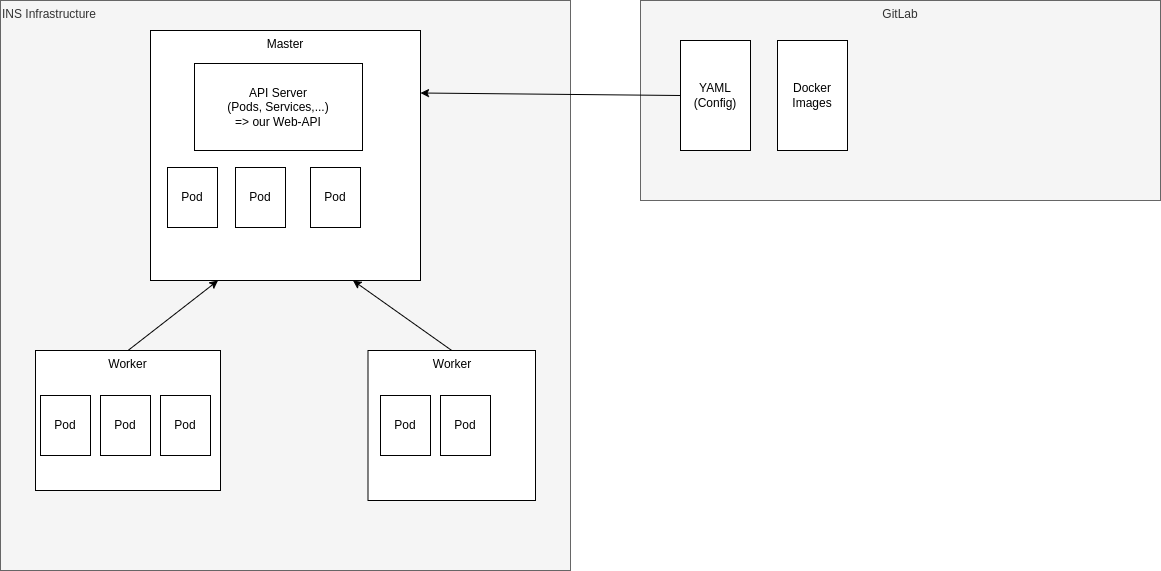
\includegraphics[height=8cm]{resources/architecture.png}
\end{figure}

\begin{figure}[h]
  \centering
  \caption{\label{fig:wireframe-dashboard}Wireframe for dashboard}
  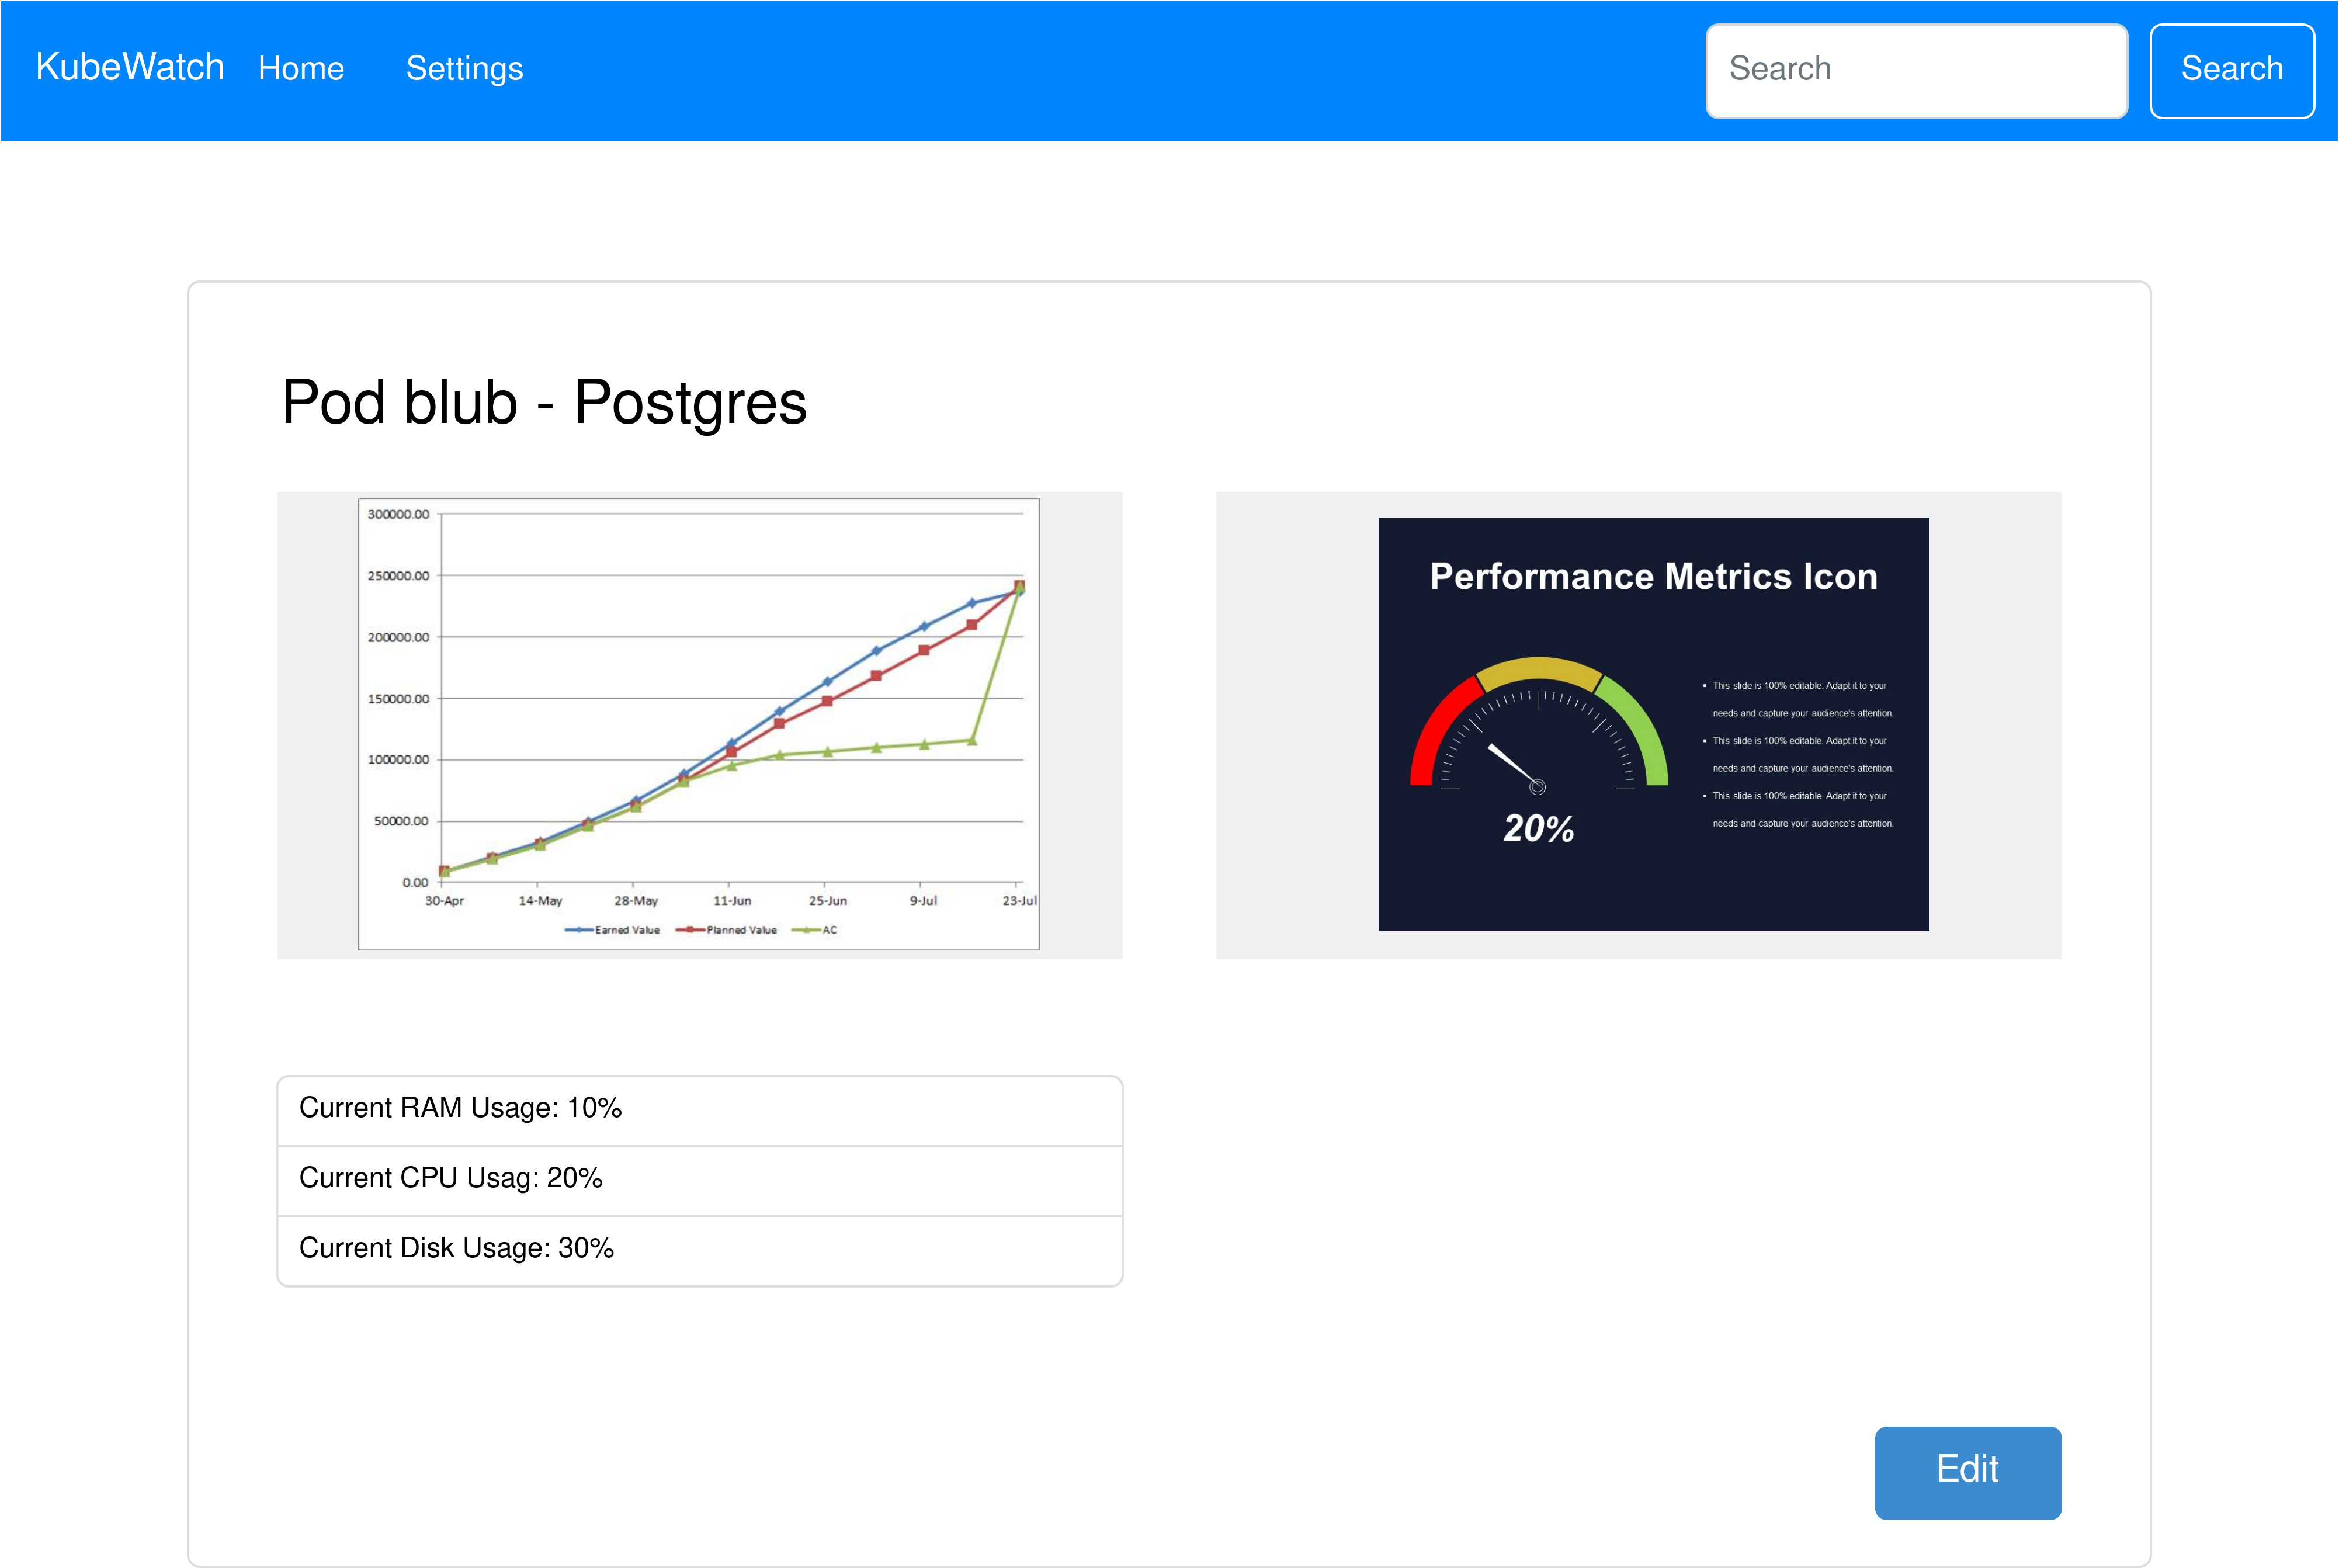
\includegraphics[height=8cm]{resources/wireframe_kubewatch-Dashboard.png}
\end{figure}

\begin{figure}[h]
  \centering
  \caption{\label{fig:wireframe-login}Wireframe for the login page}
  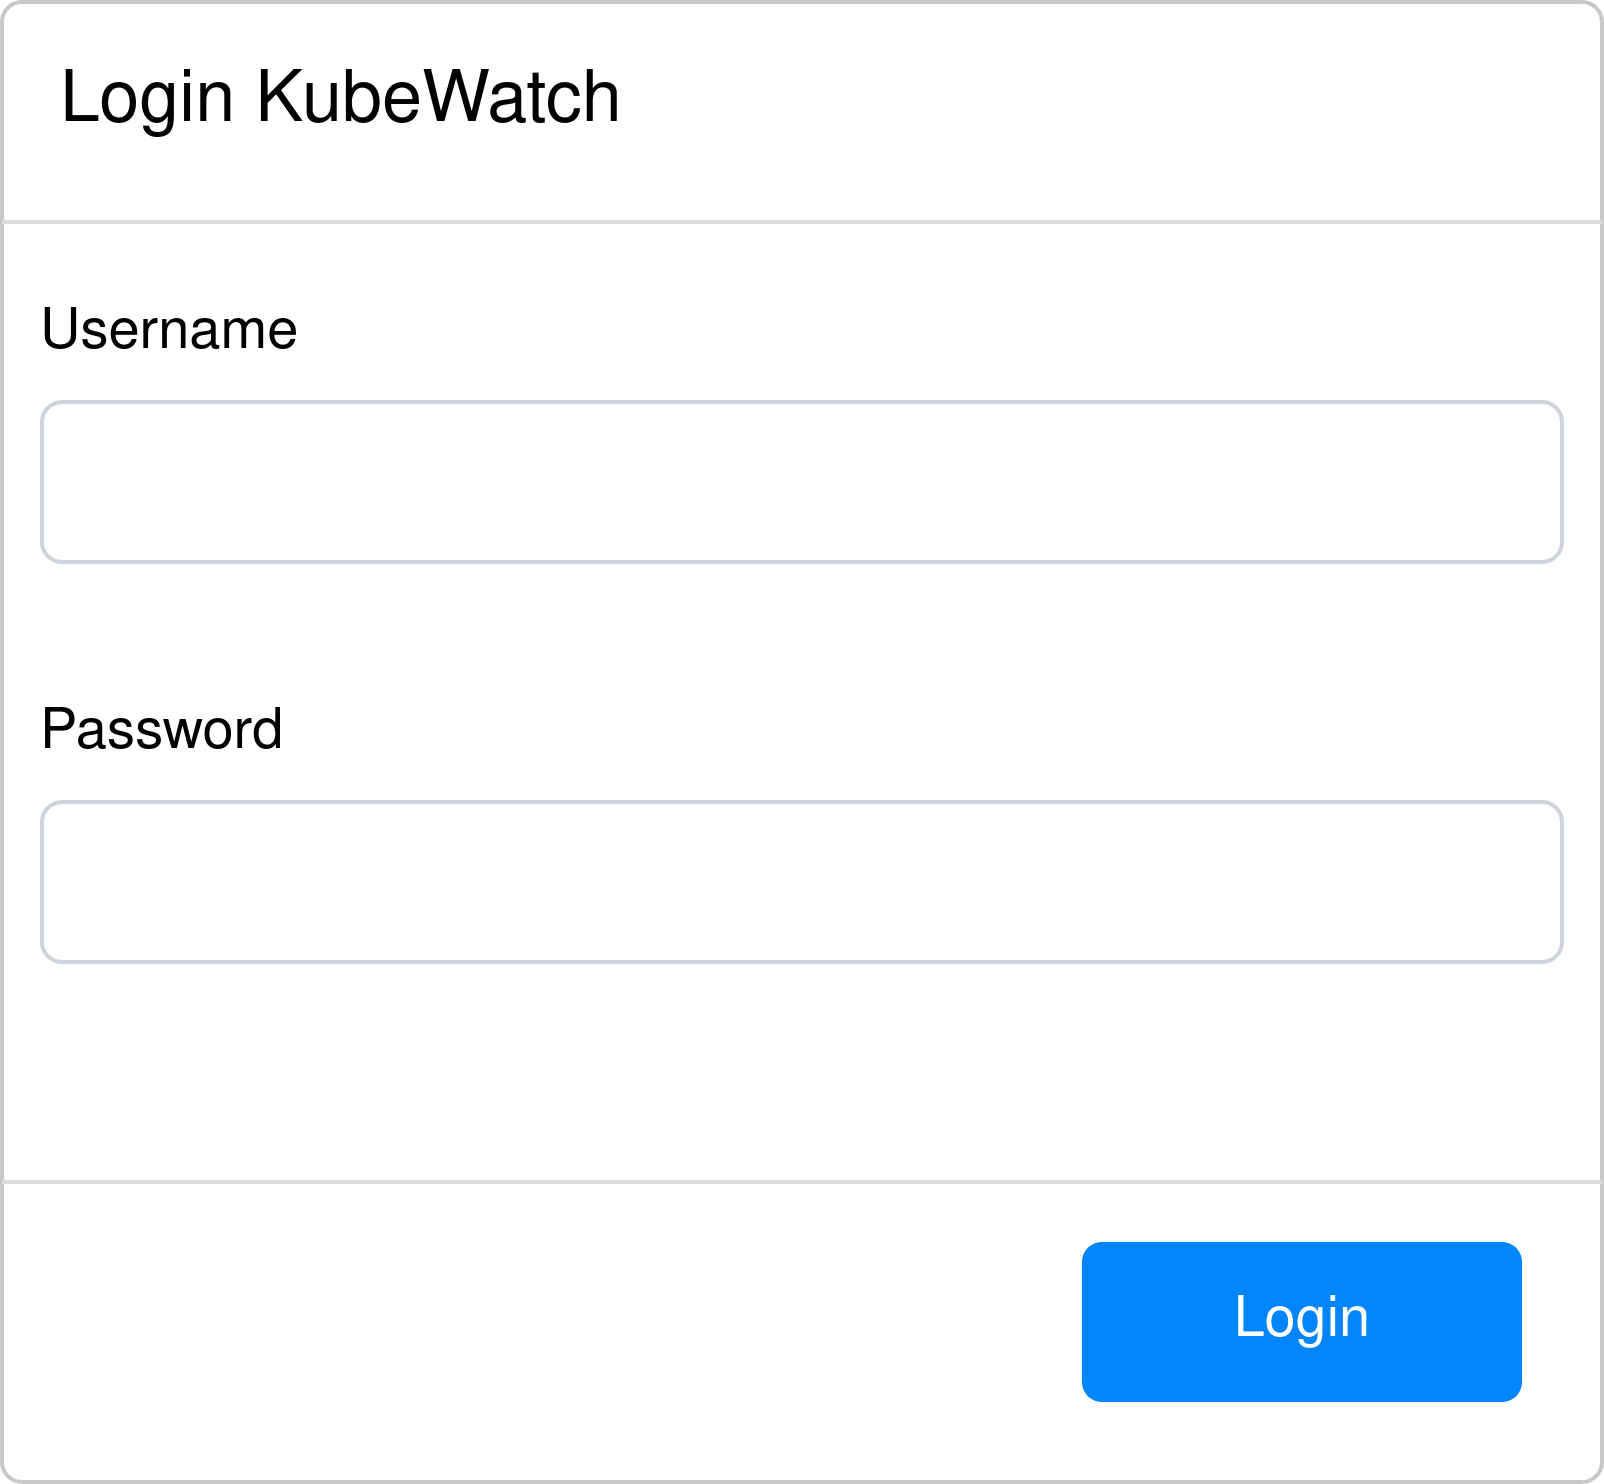
\includegraphics[height=6cm]{resources/wireframe_kubewatch-Login.png}
\end{figure}
